\documentclass{article}
\usepackage{graphicx} % Required for inserting images
\usepackage{amsmath} % Used for making newline in math expressions
\usepackage{minted}
\usemintedstyle{emacs}



\title{FYS-STK3155 Project 1}
\author{Herman Scheele, Theodor Jaarvik, Elaha Ahmadi}
\date{September 2024}

\begin{document}

\maketitle

\begin{abstract}
Linear regression is a fundamental statistical method widely employed for modeling the relationship between a dependent variable and one or more independent variables. This paper investigates the use of Ordinary Least Squares (OLS), Ridge, and Lasso regression techniques for estimating parameters in a model fitting the Franke Function and applying them to real-world terrain data. We examine the statistical properties of our data and optimal parameters, discussing the bias-variance tradeoff and employing resampling methods such as cross-validation and bootstrap to assess model performance. Our main findings indicate that both OLS and Ridge regression performed effectively on datasets of moderate complexity, with Ridge regression providing better generalization due to its regularization. Conversely, Lasso regression tended to underfit the data, likely due to excessive penalization of important features, particularly evident in the real-world terrain data where it failed to capture crucial details. These results highlight the importance of selecting appropriate regression methods and the role of regularization in handling overfitting and feature selection in datasets.
\end{abstract}



\section{Introduction}

Machine learning has become an essential tool for solving various complex problems in both academic and industrial fields. Regression analysis, in particular, plays a crucial role in modeling and predicting relationships between variables. A key challenge in regression is selecting appropriate models that balance complexity and computational cost while effectively capturing the underlying patterns in the data.
\newline\newline
In this project, we focus on regression analysis using methods such as Ordinary Least Squares (OLS), Ridge, and Lasso regression, as well as resampling techniques like bootstrap and cross-validation. Our goal is to compare the effectiveness of these different regression models and understand how resampling techniques can help in evaluating model performance, particularly in terms of the bias-variance tradeoff and overfitting prevention.
\newline\newline
We apply these models to both synthetic data generated by the Franke Function and real-world terrain data to assess their performance in different contexts. The Franke Function provides a controlled environment with known properties and adjustable noise, allowing us to evaluate how well each regression method can fit complex, nonlinear surfaces. The real-world terrain data introduces additional complexity and noise, testing the models ability to generalize to practical applications.
\newline\newline
The structure of this report is as follows: We begin by applying OLS to the Franke Function, establishing a baseline for performance. We then introduce regularization techniques with Ridge and Lasso regression to address potential overfitting issues. Then, we will derive some of the statistical interpretations of linear regression. Next, we conduct a bias-variance trade-off analysis using resampling methods to evaluate model generalization. Finally, we apply the developed models to analyze real digital terrain data, discussing the practical implications of our findings.
\newline\newline
Through this comprehensive study, we aim to provide insights into the advantages and limitations of each regression method, offering guidance on selecting appropriate techniques for different types of datasets and highlighting the importance of regularization in handling overfitting and feature selection.  



\section{Methods}





\subsection{The Franke Function}

In this study, we employ the Franke Function as a test case to evaluate the performance of various linear regression techniques, including Ordinary Least Squares (OLS), Ridge Regression, and Lasso Regression. The Franke Function is a well-known benchmark function in numerical analysis, interpolation and fitting algorithms, particularly useful for testing regression algorithms due to its nonlinear and complex structure.
\newline

The Franke function, which is a weighted sum of four exponentials reads as follows.

\begin{align*}
f(x,y) &= \frac{3}{4}\exp{\left(-\frac{(9x-2)^2}{4} - \frac{(9y-2)^2}{4}\right)} + \frac{3}{4}\exp{\left(-\frac{(9x+1)^2}{49} - \frac{(9y+1)}{10}\right)} \\
&\quad + \frac{1}{2}\exp{\left(-\frac{(9x-7)^2}{4} - \frac{(9y-3)^2}{4}\right)} - \frac{1}{5}\exp{\left(-(9x-4)^2 - (9y-7)^2\right)}.
\end{align*}
\newline
Our input functions will be defined for \(x, y \in [0,1]\). In a sense, our data are thus scaled to a particular domain for the input values. We will also add stochastic noise to our function data using the normal distribution \(\epsilon \sim N(\mu, \sigma^2)\) to simulate more realistic data. For the code implementation for our data we will be using code gathered from the FYS-STK3155 jupyter-notebook. \cite{FYS-STK3155}.
\newline

\begin{minted}[linenos, frame=lines]{python}
# Franke function definition
def FrankeFunction(x, y):
    term1 = 0.75 * np.exp(-(0.25*(9*x - 2)**2) - 0.25*((9*y - 2)**2))
    term2 = 0.75 * np.exp(-((9*x + 1)**2) / 49.0 - 0.1*(9*y + 1))
    term3 = 0.5 * np.exp(-(9*x - 7)**2 / 4.0 - 0.25*((9*y - 3)**2))
    term4 = -0.2 * np.exp(-(9*x - 4)**2 - (9*y - 7)**2)
    return term1 + term2 + term3 + term4

np.random.seed(2018)
# Define the fixed step size and generate grid points
step_size = 0.02  # Adjust this value for different step sizes
x_values = np.arange(0, 1, step_size)
y_values = np.arange(0, 1, step_size)
x_grid, y_grid = np.meshgrid(x_values, y_values)
x = x_grid.ravel()
y = y_grid.ravel()
n = len(x)

# z-values for the franke function
z = FrankeFunction(x, y) + np.random.normal(0, 1, x.shape)  # Adding Gaussian noise

\end{minted}






\subsection{Linear regression and its applications}

To fit the generated data, we employ three linear regression techniques: Ordinary Least Squares (OLS), Ridge Regression, and Lasso Regression. We will evaluate each model using the Mean Squared Error and the R2 score which reads as follows.
\begin{equation}
    \text{MSE} = \frac{1}{n} \sum_{i=1}^{n} (y_i - \hat{y}_i)^2
\end{equation}
\begin{equation}
    R^2 = 1 - \frac{\sum_{i=1}^{n} (y_i - \hat{y}_i)^2}{\sum_{i=1}^{n} (y_i - \bar{y})^2}
\end{equation}
\newline

In our study, we apply regression techniques with several key objectives. First, transforming the input variables into polynomial features allows the linear models to capture and approximate the nonlinear surface of the Franke Function. By comparing the performance of OLS, Ridge, and Lasso, we can evaluate how regularization affects model accuracy and complexity. Regularization techniques, particularly in Ridge and Lasso, are essential for preventing overfitting by striking a balance between fitting the training data and maintaining predictive performance on unseen data. Finally, Lasso Regression's inherent feature selection enhances model interpretability by identifying the most significant features, providing deeper insights into the underlying data.

\subsection{Ordinary Least Squares}
Ordinary Least Squares (OLS) regression is a fundamental statistical method used to estimate the relationship between a dependent variable and one or more independent variables. OLS aims to find the coefficient vector \(\beta\) that minimizes the sum of squared residuals between the observed values \(z\) and the predicted values \(\hat{z}\). 
The estimated coefficient vector \( \hat{\beta} \) is obtained by minimizing the sum of squared residuals:

\[
\hat{\beta} = \arg \min_{\beta} \| y - X \beta \|_2^2
\]

The closed-form solution for the Ordinary Least Squares (OLS) estimator \( \hat{\beta} \) is then given by the normal equation:


\begin{equation}
    \hat{\beta} = (X^TX)^{-1}X^Tz
\end{equation}
\newline
Where X is our design matrix and z is a vector consisting of our z values. When dealing with multidimensional surfaces like the Franke function we encounter more than one independent variable. In our case we have two, x and y. This means that we need a x and y dependence on the form \([x,y,x^2,y^2,xy,...]\) to generate a polynomial fit to the data. Our design matrix will thus be on the form 
\newline

\[
\mathbf{X} =
\begin{pmatrix}
1 & x_1 & y_1 & x_1^2 & y_1^2 & x_1 y_1 & ...\\
1 & x_2 & y_2 & x_2^2 & y_2^2 & x_2 y_2 & ...\\
1 & x_3 & y_3 & x_3^2 & y_3^2 & x_3 y_3 & ...\\
\vdots & \vdots & \vdots & \vdots & \vdots & \vdots \\
1 & x_n & y_n & x_n^2 & y_n^2 & x_n y_n & ...\\
\end{pmatrix}
\]
\newline




After finding the coefficient vector \(\hat{\beta}\), we calculate our predictive values 


\begin{equation}
    \Tilde{z} = X\hat{\beta}
\end{equation}
\newline


This is our predictive values that can be expressed as a linear combination:  
\[
\Tilde{z} = \beta_0 + \beta_1 x_1 + \beta_2 y_1 + \beta_3 x_1^2 + \beta_4 y_1^2 + \beta_5 x_1 y_1 + \cdots
\]
\newpage

In this OLS analysis we will be using polynomials in \(x\) and \(y\) up to the fifth order. Below is the code implementation of a design matrix and the calculation of the coefficient vector and the predictive values.

\begin{minted}[linenos, frame=lines, breaklines]{python}
def create_design_matrix(x, y, degree):
    X = np.ones((len(x), 1)) # Column of ones for the intercept  
    for i in range(1, degree + 1):
        for j in range(i + 1):
            X = np.column_stack((X, (x**(i-j)) * (y**j)))
    return X

# Optimal values for beta calculated with X_train and Z_train
beta = np.linalg.pinv(X_train_scaled.T @ X_train_scaled) @ X_train_scaled.T @ z_train 
betaValues.append(beta)
    
# predictive model trained and tested on training data 
model_train = X_train_scaled @ beta

# predictive model trained on training data but tested on testing data
model_test = X_test_scaled @ beta
\end{minted}
\vspace{0.7cm}


\subsubsection{Data Splitting: Training and Test sets}
To evaluate the performance of our OLS regression model, we split the dataset into training and testing subsets. This approach allows us to assess how well the model trained on one portion of the data performs on unseen data, which is crucial for detecting overfitting and ensuring that the model can generalize to new inputs. 
To implement this we utilized the \(train \_ test \_ split\) function from the scikit-learn \cite{scikit-learn} library to randomly partition the data. The dataset was divided into \(70\%\) for training and \(30\%\) for testing, a common split ratio that provides a balance between training the model effectively and having sufficient data to evaluate its performance.

\subsubsection{Scaling}
Feature scaling is a preprocessing technique used to standardize the range of independent variables or features in the data. In the context of polynomial regression, especially with higher-degree terms, scaling becomes important due to the potential for large differences in the magnitude of feature values. We applied feature scaling to the design matrix using the StandardScaler class from scikit-learn \cite{scikit-learn}. This scaler standardizes features by removing the mean and scaling to a variance of 1, resulting in a dataset where each feature has a mean of zero and a standard deviation of 1. This also means that our intercept column becomes a zero vector and we can disregard \(\beta_0.\)

\subsubsection{Why Scale the data?}
Firstly, scaling helps prevent numerical issues that can arise during matrix computations, such as inversion, especially when dealing with polynomial terms of varying magnitudes. Secondly, features with larger scales can negatively impact the model. Scaling ensures that each feature contributes equally to the model's learning process. Finally, for optimization algorithms, scaled data can lead to faster running times to find the optimal values.

\subsection{Ridge Regression}
Ridge regression is an extension of the OLS method that incorporates a regularization term to mitigate the effects of overfitting, especially in situations where the design matrix \(X\) contains multicollinear or highly correlated features. Ridge regression adds a penalty term to the OLS cost function. This penalty term effectively shrinks the magnitude of the coefficients, resulting in a more stable and generalizable model.
\newline

The Ridge regression cost function is defined as:

\[
J(\beta) = \frac{1}{2N} \sum_{i=1}^{N} (y_i - \hat{y}_i)^2 + \lambda \sum_{j=1}^{p} \beta_j^2
\]

Here, \( \lambda \) is a hyperparameter that controls the strength of regularization. A larger \( \lambda \) increases the penalty on large coefficients, while a smaller \( \lambda \) reduces the impact of the regularization term, approaching the OLS solution as \( \lambda \to 0 \).
\newline\newline
The closed-form solution for the Ridge regression estimator is given by:

\[
\hat{\beta}_{\text{ridge}} = (X^TX + \lambda I)^{-1} X^T y
\]

Where \(I\) is the identity matrix, and \( \lambda \) is the regularization parameter.

\subsubsection{Implementation of Ridge Regression}

In our implementation, we used the Franke Function to generate the dataset, adding a small amount of noise to simulate real-world data. The polynomial design matrix was created with terms up to the fifth degree in \(x\) and \(y\), ensuring that the model could capture the nonlinear surface of the Franke function.
\newpage

The following steps outline our Ridge regression process:

\paragraph{1. Data Preparation and Feature Scaling:}
As with OLS, the design matrix was standardized using the `StandardScaler` from the scikit-learn library to ensure that each feature contributed equally to the model. Scaling the features is particularly important in Ridge regression because it prevents features with larger magnitudes from dominating the regularization term.

\paragraph{2. Ridge Regression Estimator:}
The Ridge regression estimator was implemented using the following function, where the regularization parameter \( \lambda \) was varied across multiple values to analyze its impact on the model performance.

\begin{minted}[linenos, frame=lines, breaklines]{python}
def RidgeRegression(X_train, z_train, X_test, lmbda):
    I = np.eye(X_train.shape[1])  # Identity matrix
    beta_ridge = np.linalg.pinv(X_train.T @ X_train + lmbda * I) @ X_train.T @ z_train
    z_pred = X_test @ beta_ridge
    return z_pred, beta_ridge
\end{minted}

\paragraph{3. Model Evaluation:}
We evaluated the Ridge regression models using the MSE and the R2 score across different values of \( \lambda \), ranging from 0.01 to 100. This allowed us to explore the tradeoff between bias and variance in Ridge regression. As \( \lambda \) increases, the model becomes less sensitive to the training data, reducing variance but potentially increasing bias.




\paragraph{4. Validation and Model Selection:}
To ensure the validity of our Ridge regression model, we compared the results at \( \lambda = 0.01 \) to the OLS solution, observing that the results converged as expected. Additionally, cross-validation could be implemented to further assess the generalization performance of the model and fine-tune the regularization parameter \( \lambda \).
\newline


\subsection{Lasso Regression}

Lasso regression, like OLS regression, aims to minimize the difference between predicted and true values. However, it introduces an additional L1 regularization term in its cost function, which penalizes large coefficients. This regularization can shrink some coefficients to exactly zero, effectively eliminating irrelevant features. This makes Lasso particularly useful for datasets with many features, helping in both feature selection and reducing overfitting.  
\newpage

Lasso cost loss function:
    
\begin{align*}
    J(\beta) = \frac{1}{2N} \sum_{i=1}^{N} \left( y_i - \hat{y}_i \right)^2 + \lambda \sum_{j=1}^{p} |\beta_j|\\
\end{align*}

This project implements \cite{scikit-learn} Scikit-learn's lasso regression, where the parameters of the function are changed to fit the dataset. Below is an example of the code implementation:\\\\

    \includegraphics[width=1\linewidth]{imageLasso.png}\\\\
    \caption{\cite{scikit-learn} Scikit-learn: Lasso regression}
    \label{fig:enter-label}\\\\

The max iter parameter defines the maximum number of iterations allowed for the optimization algorithm to converge. The alpha parameter, equivalent to \(\lambda\) in the cost function, controls the strength of the regularization. A higher alpha value increases the regularization penalty, shrinking the coefficients of less important features toward zero, effectively performing feature selection. When alpha is set to 0, the regularization term is removed, and the model behaves like standard OLS regression. The visualization below shows the interconnection between increasing values of alpha and the \(\beta\) coefficients.  \\\\

    
    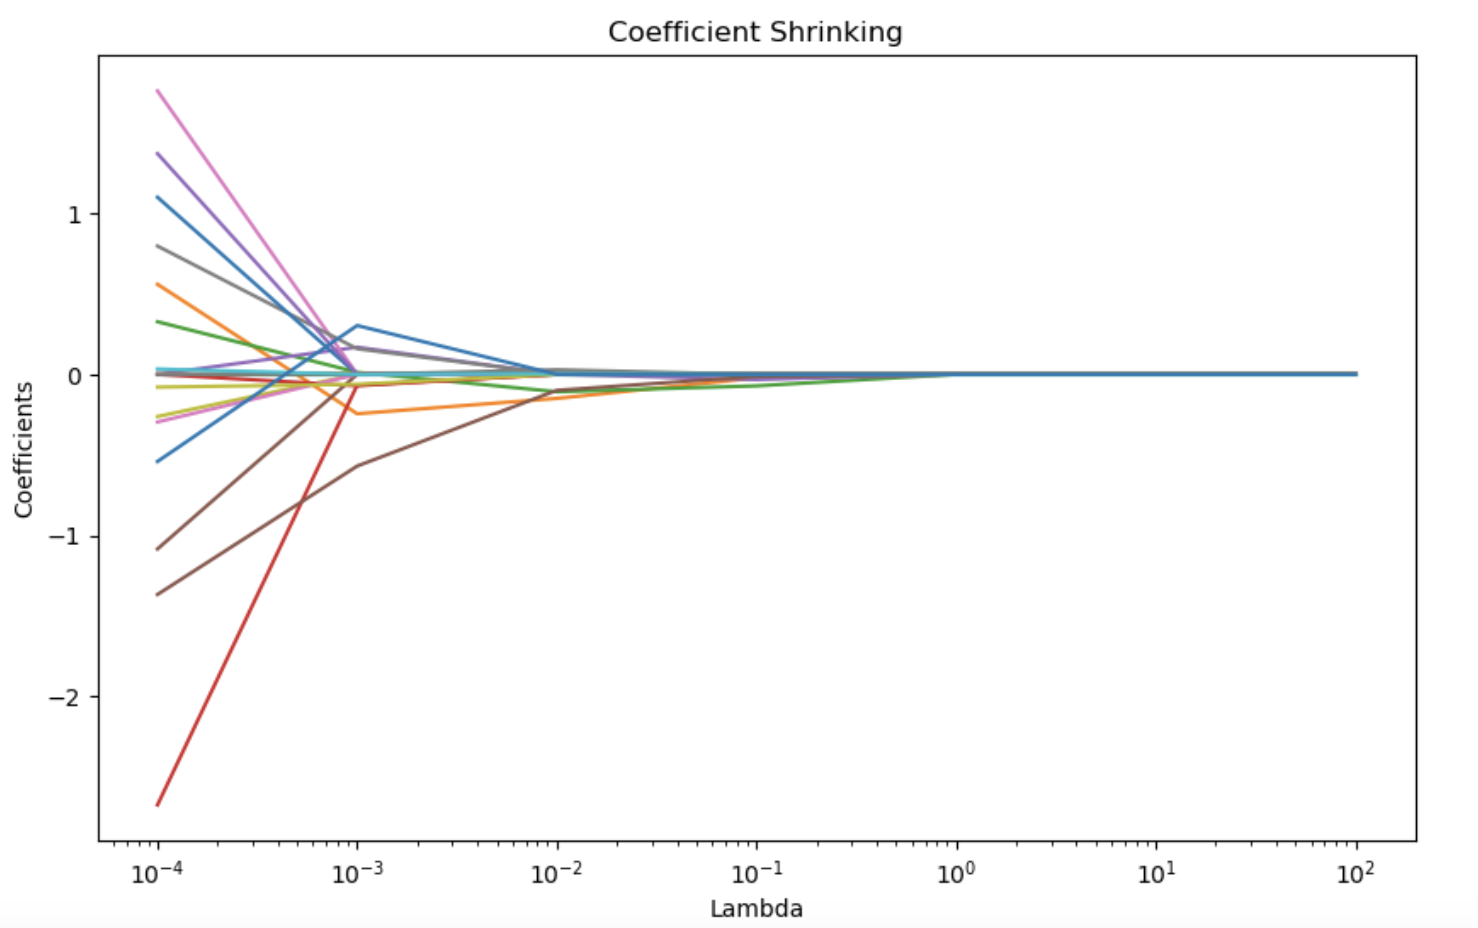
\includegraphics[width=1\linewidth]{imageLassoShrinkage.png}
    \caption{Figure 1: Coefficient shrinking for different values of lambda}
    \label{fig:enter-label}\\\\
    


\subsubsection{Impact of \(\lambda\) on \(\beta\) Coefficients in Ridge Regression}

In Ridge regression, the coefficients \(\beta\) are estimated by minimizing:

\[
\hat{\beta}_{ridge} = \arg\min \left( ||\mathbf{y} - \mathbf{X}\beta||^2 + \lambda ||\beta||^2 \right).
\]

As \(\lambda\) increases, the regularization term \(\lambda ||\beta||^2\) penalizes large coefficients, shrinking \(\beta\) towards zero. For \(\lambda = 0\), Ridge regression reduces to OLS, but as \(\lambda \to \infty\), \(\beta\) tends to zero, leading to a simpler model with higher bias but lower variance. Thus, \(\lambda\) balances model complexity by controlling the magnitude of \(\beta\) and mitigating overfitting. \\\\


\subsection{Statistical interpretation of Linear Regression}
The analysis begins with the linear model assumption, where the relationship between the observed data \(y\) and the true underlying function \(f(x)\) is given by:
\[
y = f(x) + \epsilon
\]

Here, \( \epsilon \sim N(0, \sigma^2) \) represents normally distributed noise with mean 0 and variance \( \sigma^2 \). The function \( f(x) \) is approximated using a linear model \( \hat{y} = X\beta \), where \( X \) is the design matrix, \( \beta \) represents the vector of parameters, and \( \hat{y} \) is the predicted value. The parameters \( \beta \) are estimated using the OLS method by minimizing the resudual sumof squares: \[
\hat{\beta} = (X^TX)^{-1}X^Ty
\]
\newline



\subsubsection{Expectation Value of \(\hat{y}_i\)}

The predicted response \(\hat{y}_i\) is given by:

\[
\hat{y}_i = \mathbf{x}_i^\top \hat{\beta}
\]

The expectation of \(\hat{y}_i\) is:

\[
\mathbb{E}[\hat{y}_i] = \mathbb{E}[\mathbf{x}_i^\top \hat{\beta}] = \mathbf{x}_i^\top \mathbb{E}[\hat{\beta}]
\]

Since \(\mathbb{E}[\hat{\beta}] = \beta\), it follows that:

\[
\mathbb{E}[\hat{y}_i] = \mathbf{x}_i^\top \beta
\]
\newline

\subsubsection{Variance of \(\hat{y}_i\)}


We assume the model \( y_i = \mathbf{x}_i^\top \beta + \epsilon_i \), where \( \epsilon_i \sim N(0, \sigma^2) \). \\\\

Since \(\mathbf{x}_i^\top \beta\) is deterministic and \(\epsilon_i\) is normally distributed with variance \(\sigma^2\), we have:

\[
\text{Var}(y_i) = \text{Var}(\mathbf{x}_i^\top \beta + \epsilon_i) = \text{Var}(\epsilon_i) = \sigma^2
\]
\newline

\subsubsection{Expectation value of \(\hat{\beta}\)}

To compute the expectation and variance of \( \hat{\beta} \), substitution of \( y = X\beta + \epsilon \) into the OLS estimator is performed, and the properties of expectation and variance are applied. The expectation \( E(\hat{\beta}) \) and variance \( Var(\hat{\beta}) \)  are derived as follows:
\newline

We start with the ordinary least squares (OLS) estimator for \(\beta\):

\[
\hat{\beta} = (X^\top X)^{-1} X^\top y
\]

Assuming the model is \( y = X\beta + \epsilon \), where \(\epsilon\) is the error term with \(\mathbb{E}[\epsilon] = 0\), we substitute \( y \) into the expression for \(\hat{\beta}\):

\[
\hat{\beta} = (X^\top X)^{-1} X^\top (X\beta + \epsilon)
\]

Expanding this expression:

\[
\hat{\beta} = (X^\top X)^{-1} (X^\top X \beta + X^\top \epsilon)
\]

Since \( (X^\top X)^{-1} X^\top X = I \), we simplify to:

\[
\hat{\beta} = \beta + (X^\top X)^{-1} X^\top \epsilon
\]

Now, take the expectation of \(\hat{\beta}\):

\[
\mathbb{E}[\hat{\beta}] = \mathbb{E}\left[\beta + (X^\top X)^{-1} X^\top \epsilon\right]
\]

Since \(\beta\) is constant, we get:

\[
\mathbb{E}[\hat{\beta}] = \beta + \mathbb{E}\left[(X^\top X)^{-1} X^\top \epsilon\right]
\]

Given that \(\mathbb{E}[\epsilon] = 0\), the second term vanishes:

\[
\mathbb{E}[\hat{\beta}] = \beta
\]
\newline





\subsubsection{Variance of \(\hat{\beta}\)}

We start with the OLS estimator for \(\hat{\beta}\):

\[
\hat{\beta} = (X^\top X)^{-1} X^\top y
\]

Substituting the model \( y = X\beta + \epsilon \), we have:

\[
\hat{\beta} = (X^\top X)^{-1} X^\top (X\beta + \epsilon)
\]

Expanding this:

\[
\hat{\beta} = \beta + (X^\top X)^{-1} X^\top \epsilon
\]

To calculate the variance of \(\hat{\beta}\), we consider only the second term since \(\beta\) is constant:

\[
\text{Var}(\hat{\beta}) = \text{Var}\left( (X^\top X)^{-1} X^\top \epsilon \right)
\]

Since \((X^\top X)^{-1} X^\top\) is constant, we can factor it out of the variance:

\[
\text{Var}(\hat{\beta}) = (X^\top X)^{-1} X^\top \text{Var}(\epsilon) X (X^\top X)^{-1}
\]

By assumption, \(\epsilon \sim N(0, \sigma^2 I)\), so the variance of \(\epsilon\) is:

\[
\text{Var}(\epsilon) = \sigma^2 I
\]

Substituting this into the variance expression for \(\hat{\beta}\):

\[
\text{Var}(\hat{\beta}) = (X^\top X)^{-1} X^\top (\sigma^2 I) X (X^\top X)^{-1}
\]

Since \( X^\top X (X^\top X)^{-1} = I \), the expression simplifies to:

\[
\text{Var}(\hat{\beta}) = \sigma^2 (X^\top X)^{-1}
\]
\newline



\subsubsection{For Ridge}
In Ridge regression, the OLS estimation is modified by introducing a regularization parameter \( \lambda \), which controls the magnitude of the coefficients. The Ridge regression estimator is defines as: 
\[
\hat{\beta}_{\text{Ridge}} = (X^TX + \lambda I)^{-1}X^Ty
\]

The expectation and variance of \( \hat{\beta}_{\text{Ridge}} \) are analyzed by substituting \( y = X\beta + \epsilon \) into the estimator and applying the properties of expectation and variance operator. The expectation and variance of Ridge regression estimator are: 
\[
E(\hat{\beta}_{\text{Ridge}}) = (X^TX + \lambda I)^{-1}(X^TX)\beta
\]

\[
Var(\hat{\beta}_{\text{Ridge}}) = \sigma^2(X^TX + \lambda I)^{-1}X^TX(X^TX + \lambda I)^{-1}
\]

The effect of increasing \( \lambda \)  on the variance is also considered. As \( \lambda \to \infty \), the variance of \( \hat{\beta}_{\text{Ridge}} \) tends to zero, but the bias increases demonstrating the bias-variance trade-off in Ridge regression.  
\newline


\subsection{Bias-Variance Tradeoff}

Understanding the bias-variance tradeoff is crucial in developing models that generalize well to new data. In the context of regression analysis, particularly when using polynomial models, the complexity of the model can significantly impact both the bias and variance of the predictions. Our goal was to analyze how varying the complexity of our models affects their bias and variance components.

\subsubsection{Model Complexity Variation}

We varied the degree of the polynomial features in our design matrix, ranging from 1 to 20. For each degree, we constructed the design matrix X using the method described earlier and fitted the models using Ordinary Least Squares regression.

\subsubsection{Resampling with Bootstrap}

To estimate the bias and variance components of our models, we employed the bootstrap resampling method. Bootstrap allows us to approximate the sampling distribution of a statistic by resampling with replacement from the original dataset.

\paragraph{Procedure}

The steps for the bootstrap method are as follows:

\begin{enumerate} 
\item \textbf{Generate Bootstrap Samples:}
For each of bootstrap iterations, we will be using 100 iterations: 
                    \begin{enumerate} 
                     \item Sample n data points with replacement from the original           dataset to create a bootstrap sample. 
                     \item Fit the regression model on the bootstrap sample. 
                     \item Predict on the original input data to obtain predictions. These predictions are used to estimate the bias and variance.
                    \end{enumerate}
                        
\item \textbf{Compute Average Predictions:}
Calculate the mean prediction for each data point across all bootstrap samples.

\item \textbf{Compute Overall Metrics:} Calculate the mean squared error (MSE), bias squared, and variance over all data points. The expected squared error can be rewritten as a term which contains the bias and variance of the model itself as shown below


\subsubsection{Bias-Variance Decomposition Derivation \cite{Elements_statistical_learning} }

The goal is to derive the decomposition of the expected squared error into bias, variance, and noise. We want to show that:

\[
E[(y - \tilde{y})^2] = \text{Bias} + \text{Variance} + \sigma^2
\]

where:
- $\text{Bias} = E[(y - E[\tilde{y}])^2]$
- $\text{Variance} = E[(\tilde{y} - E[\tilde{y}])^2]$
- $\sigma^2$ is the irreducible noise.

### Step 1: Expand the squared term
Starting with the expected squared error:

\[
E[(y - \tilde{y})^2]
\]

We expand the squared term:

\[
E[(y - \tilde{y})^2] = E[y^2 - 2y\tilde{y} + \tilde{y}^2]
\]

This can be split into three terms:

\[
E[y^2] - 2E[y\tilde{y}] + E[\tilde{y}^2]
\]

### Step 2: Add and subtract $E[\tilde{y}]$
\newline\newline
We introduce the expected value of $\tilde{y}$ into the expression:

\[
E[(y - \tilde{y})^2] = E[(y - E[\tilde{y}] + E[\tilde{y}] - \tilde{y})^2]
\]

Expanding this gives:

\[
E[(y - E[\tilde{y}])^2 + 2(y - E[\tilde{y}])(\tilde{y} - E[\tilde{y}]) + (\tilde{y} - E[\tilde{y}])^2]
\]

### Step 3: Simplify the cross term
\newline\newline
The cross term $E[2(y - E[\tilde{y}])(\tilde{y} - E[\tilde{y}])]$ becomes zero because $E[\tilde{y}]$ is a constant and independent of $y$:

\[
E[2(y - E[\tilde{y}])(\tilde{y} - E[\tilde{y}])] = 0
\]

Thus, we are left with:

\[
E[(y - \tilde{y})^2] = E[(y - E[\tilde{y}])^2] + E[(\tilde{y} - E[\tilde{y}])^2]
\]

### Step 4: Add the irreducible noise term
\newline\newline
The term $E[(y - E[\tilde{y}])^2]$ represents the bias squared, and $E[(\tilde{y} - E[\tilde{y}])^2]$ represents the variance. Additionally, there is an irreducible noise term, $\sigma^2$, which accounts for the variance in the observations around the true values.

Thus, we obtain the final bias-variance decomposition:

\[
E[(y - \tilde{y})^2] = \text{Bias}^2 + \text{Variance} + \sigma^2
\]

where:
- $\text{Bias} = E[(y - E[\tilde{y}])^2]$
- $\text{Variance} = E[(\tilde{y} - E[\tilde{y}])^2]$
- $\sigma^2$ is the irreducible error (noise).





\subsubsection{Implementation Details}

We implemented the bootstrap bias-variance estimation using Python and the following libraries:

\begin{itemize} \item \texttt{NumPy} for numerical computations. \item \texttt{scikit-learn} for regression models and resampling utilities. \cite{scikit-learn} \end{itemize}

The core implementation is as follows:

\begin{minted}[linenos, frame=lines, breaklines]{python} 

# Create an empty array to store bootstrap predictions
    z_pred = np.empty((z_test.shape[0], n_bootstraps))

    for i in range(n_bootstraps):
        # Resample the training data
        X_, z_ = resample(X_train, z_train)
        z_pred[:, i] = model.fit(X_, z_).predict(X_test).ravel()

    # Reshape z_test for broadcasting
    z_test_reshaped = z_test[:, np.newaxis]  # Shape (n_samples, 1)

    # Calculate bias, variance, and error
    error[degree] = np.mean((z_test_reshaped - z_pred) ** 2)
    mean_z_pred = np.mean(z_pred, axis=1)  # Shape (n_samples,)
    bias[degree] = np.mean((z_test - mean_z_pred) ** 2)
    variance[degree] = np.mean(np.var(z_pred, axis=1))
\end{minted}






\subsection{Cross-validation resampling (f)}

Cross-validation resampling is a technique used to enhance the generalization of a model while minimizing the risk of overfitting. This method involves repeatedly splitting the dataset into training and testing subsets, allowing for a more robust evaluation of the model’s performance. The parameter \(k\) specifies the number of folds in the cross-validation process, determining how many distinct iterations of the dataset are generated.\\

In each iteration, the dataset is divided into \(k\)  subsets, or folds. One fold is reserved for testing, while the remaining \(k-1\)  folds are utilized for training the model. This process is repeated \(k\)  times, ensuring that each fold serves as the test set exactly once. By employing this approach, cross-validation creates a series of varied test-train splits, resulting in a comprehensive assessment of the model’s ability to generalize across different data segments.\\

Cross-validation was integrated into the project using \cite{scikit-learn} Scikit-learn’s \(cross val score \)  along with the MSE scorer. This implementation was applied in conjunction with Scikit-learn’s Ordinary Least Squares (OLS), Ridge, and Lasso regression models. As the custom regression algorithms were not coded to accommodate cross-validation, this integration allowed for the generation of MSE scores for each regression method. The mean of these scores was then utilized for visualization, providing insights into the performance and accuracy of the different regression techniques. Below is the code for implementation.\\

\includegraphics[width=1\linewidth]{imageCrossVal.png}
\caption{Code: \cite{scikit-learn} Cross validation implementation using scikit}
\label{fig:enter-label}\\

This piece of code will run the k-fold cross validation 5 times, one time for each \( k \in [5,10]\), resulting in an output of MSE-scores for OLS, Ridge and Lasso regression for each \(k\). This was done in order to analyse how higher values of \(k\) affect the MSE-score, as well as ensuring the models were not overfitted. The visualization below shows a typical run of the cross-validation code.\\


\includegraphics[width=1\linewidth]{imageCrossValMSE.png}
\caption{Figure 2: Cross-validation: MSE for different values of k}
\label{fig:enter-label}


   




\subsection{Analysis of real data}

\subsubsection{Data Preprocessing}

The real-world terrain data from Norway, provided in \texttt{.tif} format, was loaded using the \texttt{imread} function from the \texttt{imageio} library and visualized as a 2D grayscale image. To prepare the data for regression, we flattened the 2D grid coordinates into 1D arrays and introduced noise to simulate real-world conditions:

\includegraphics[width=1\linewidth]{1.png}
\caption{Code: Preparing the data }
\label{fig:enter-label}\\\\


\subsubsection{Polynomial Design Matrix}

We applied polynomial regression by constructing a \textit{design matrix} that includes polynomial terms up to degree 5. This design matrix allows the model to fit more complex surfaces to the terrain data. The following function constructs the design matrix for our 2D grid:

\includegraphics[width=1\linewidth]{2.png}
\caption{Code: Design matrix }
\label{fig:enter-label}\\\\


\subsubsection{Data Standardization and Train-Test Split}

Since Ridge and Lasso are sensitive to the scale of input data, we standardized the design matrix so that all features have a mean of 0 and a standard deviation of 1. We also split the data into training (70\%) and testing (30\%) sets:


\includegraphics[width=1.3\linewidth]{3.png}
\caption{}
\label{fig:enter-label}\\\\
\includegraphics[width=1\linewidth]{4.png}
\caption{Code: Train-test split }
\label{fig:enter-label}\\\\


\subsubsection{Model Implementation}

We implemented three regression models: \textit{Ordinary Least Squares (OLS)}, \textit{Ridge}, and \textit{Lasso}. These models were fitted to the standardized training data, and their performance was evaluated based on the \textit{Mean Squared Error (MSE)} on the test set \cite{james2013introduction}. The core implementation is as follows:


\includegraphics[width=1\linewidth]{5.png}
\caption{Code: Implementations }
\label{fig:enter-label}\\\\



\subsubsection{Model Evaluation: MSE Calculation}

After fitting the models, we used the test set to evaluate their performance by calculating the MSE. Lower MSE values indicate better performance, as they measure how closely the predicted terrain heights match the actual data.

\includegraphics[width=1\linewidth]{6.png}
\caption{Code: MSE calculation }
\label{fig:enter-label}\\\\


\subsubsection{Cross-Validation with K-Fold}

To ensure the models generalized well across different parts of the data, we used \textit{5-Fold Cross-Validation}. This technique splits the training data into 5 subsets, fits the model on 4 subsets, and validates it on the remaining subset. This process is repeated 5 times, with each fold serving as the validation set once. The average MSE across the 5 folds was computed to assess model stability.

\includegraphics[width=1\linewidth]{7.png}
\caption{Code: Cross-validation }
\label{fig:enter-label}\\\\


\subsubsection{Visualization of Results}

To better interpret the results, we visualized both the original terrain and the terrain predicted by the OLS model. This was done using 3D surface plots, which allowed us to compare the complexity of the original terrain to the model’s predicted surface.

\includegraphics[width=1\linewidth]{8.png}
\caption{Code: Visualization }
\label{fig:enter-label}\\\\

In summary, we implemented polynomial regression models (OLS, Ridge, and Lasso) and evaluated their performance using MSE and cross-validation. The visualization confirmed that while OLS and Ridge performed similarly, both failed to capture the detailed complexity of the terrain, and Lasso performed worse due to oversimplification. Cross-validation provided further confirmation that Ridge did not significantly outperform OLS.



\section{Results}

Github: https://github.com/TheodorJaarvik/Fys-stk3155\_Project-1

\subsection{Ordinary Least Squares Regression Results}


\subsubsection{Model Performance Metrics}
The table below visually descirbes how the MSE and R2 score changes as model complexity increases. 

   
    \begin{center}
    \includegraphics[width=1.3\linewidth]{OLS_MSE_R2.png}
    \caption{Figure 3: MSE and R2 score change as polynomial degree increases}
    \label{fig:enter-label}
    \end{center}
    

This summarizes the MSE and R2 scores for the OLS model at different polynomial degrees ranging from 1 to 5. These metrics provide insights into how well the model fits the training data and how it generalizes to unseen data.


As observed, the training MSE decreases with increasing polynomial degree, indicating that the model fits the training data more closely. The training R2 score also increases, which signifies a better fit. However, the test MSE does not decrease at the same rate, and the test R2 score shows diminishing returns beyond a polynomial degree of 4. This suggests that while the model is improving its fit on the training data, its ability to generalize to unseen data does not improve proportionally, hinting at potential overfitting at higher degrees.

\subsubsection{Beta Coefficients and Polynomial Degree}
In our analysis we also plotted the beta coefficients as a function of model complexity. The following plot visualizes how the coefficients change with higher polynomial degrees.

    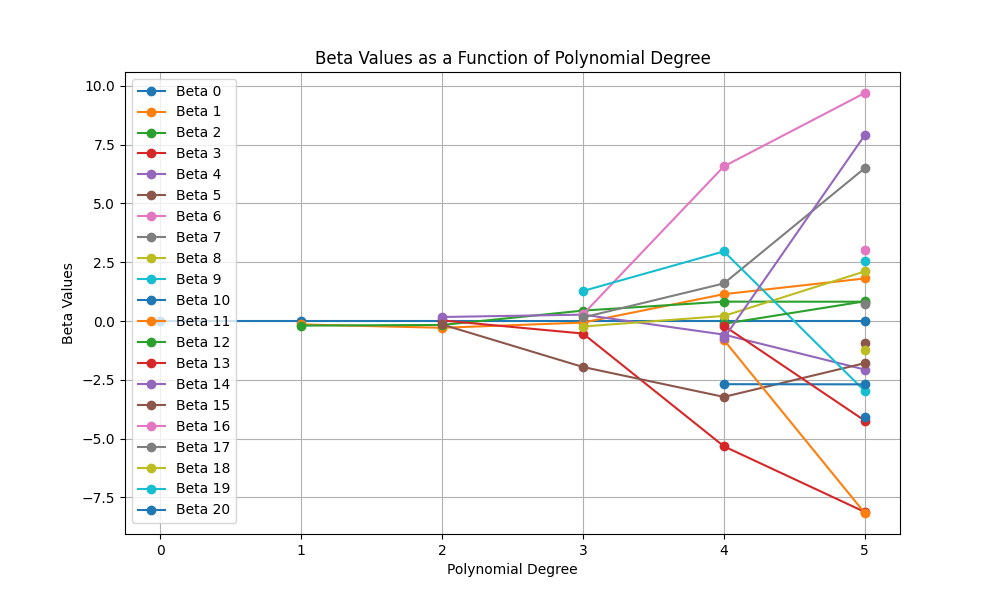
\includegraphics[width=1\linewidth]{beta_values.png}
    \caption{Figure 4: Coefficient change with polynomial degree increase}
    \label{fig:enter-label}\\\\


The beta coefficients in Ordinary Least Squares regression evolve significantly as the degree of the polynomial increases, as shown above. For lower degrees (0 to 2), the coefficients remain small and close to zero, indicating a stable model with limited complexity.

However, beyond degree 2, the coefficients for higher-order terms diverge, with some increasing sharply, while others show strong negative trends. This reflects the model's increasing flexibility as it adapts to the data, often at the cost of overfitting, as indicated by large coefficient magnitudes.

The growing volatility in $\beta$ values with higher polynomial degrees highlights the trade-off between bias and variance, where reduced bias leads to increased sensitivity to data noise. Controlling this effect is essential to avoid overfitting, especially when dealing with complex models.


\subsubsection{Comparison with Scikit-Learn Implementation}

To validate the correctness of our manual OLS implementation, we compared the results with those obtained using the OLS model from the scikit-learn library \cite{scikit-learn}. The figure below illustrates the comparison of the MSE values from both implementations across different polynomial degrees.


\includegraphics[width=1.3\linewidth]{OLS_comparisons.png} 
\caption{Figure 5: Comparison with \cite{scikit-learn} scikit learn implementation}
\label{fig} \\


The identical MSE values between our manual model and a scikit learn model confirm that our OLS implementation is consistent with the standard library function, thus validating the accuracy of our code.

\subsubsection{Visualizing the Model Fit}

To assess how well the OLS model captures the underlying structure of the Franke Function, we visualized the predicted surface alongside the true datapoints. The figure below shows the data point plots of the Franke Function and the OLS-predicted values using a fifth-degree polynomial.

    \includegraphics[width=1\linewidth]{dp_surface.png}
    \caption{Figure 6: OLS-model compared to Franke-function, fifth-degree polynomial}
    \label{fig:enter-label}\\\\


The OLS model with a fifth-degree polynomial captures the main features of the Franke Function, including the peaks and valleys. Notice that this visualization is of a Franke function that has no added noise to it. With a perfectly distributed Franke function, we still notice some discrepancies, indicating that while the model performs well, there is room for improvement in capturing finer details.


\subsubsection{Impact of noise}
In our main OLS implementation we fitted a model to the Franke Function with added noise that is normally distributed. As we can tell form the graph that described the MSE and R2 scores as a function of model complexity we observe high values for MSE and R2 relative to the numerical intervals our independent variables operate in. We analysed this by reducing the gaussuian noise added to the Franke Function by a factor of ten (0.1). The graph below descirbes the same relation with model complexity but with significantly lower values of MSE.  


    \includegraphics[width=1\linewidth]{less_noise_OLS_mse.png}
    \caption{Figure 7: MSE and R2 score with less noise}
    \label{fig:enter-label}\\\\

\subsubsection{Effect of data amount and distribution}

As we can observe in the graph above, the test and training values are almost identical when we reduce the noise. This implies that our model is fitting extremely well on testing data. This can be explained by the fact that the original independent variables x and y are evenly distributed in a grid using the following code: 

\begin{minted}[linenos, frame=lines, breaklines]{python} 
    # Define the fixed step size and generate grid points
    step_size = 0.02  # Adjust this value for different step sizes
    x_values = np.arange(0, 1, step_size)
    y_values = np.arange(0, 1, step_size)
    x_grid, y_grid = np.meshgrid(x_values, y_values)
    x = x_grid.ravel()
    y = y_grid.ravel()
\end{minted}

When our data is distributed evenly and we have a large amount of it, our model captures the underlying features of the true data very well and this is reflected by the fact that there is a minuscule difference between the testing and training error values.

\subsubsection{Effect of Feature Scaling}

Feature scaling proved to be a crucial step in our analysis. Without scaling, the OLS model would experience numerical instability due to the large differences in the magnitudes of the polynomial features, especially at higher degrees. By applying standardization, we ensured that all features contributed equally to the model, which improved the numerical stability and convergence of the model fitting process.

\subsubsection{Overfitting and Model Complexity}

As we increased the complexity of the model, we observed that the training and test MSE continued to decrease. If we were to introduce higher complexity, and or fewer data points, less evenly distributed data and more Gaussian noise, we would observe a divergence between the training and testing MSE values. The widening gap would indicate that the model is overfitting to the training data including its noise, which adversely affects its generalization to new data. 
\newline

Our findings highlight the importance of selecting an appropriate polynomial degree to balance the trade-off between bias and variance. The validation against scikit-learn's implementation confirms the correctness of our manual OLS approach.



\subsection{Results for Ridge regression}

In this section, we present the results obtained from the Ridge regression analysis applied to the data generated by the Franke Function. As outlined in the methods section, we varied the regularization parameter \( \lambda \) to observe its effect on the model's performance in terms of Mean Squared Error (MSE) and \(R^2\) score for both the training and test sets.

\subsection{Effect of Regularization on Model Performance}

To investigate the effect of regularization, we tested multiple values of \( \lambda \) in the range from 0.01 to 100. The resulting training and test errors, as measured by MSE and R2, are displayed in the graph below. The results highlight the tradeoff between bias and variance in Ridge regression as \( \lambda \) increases.


    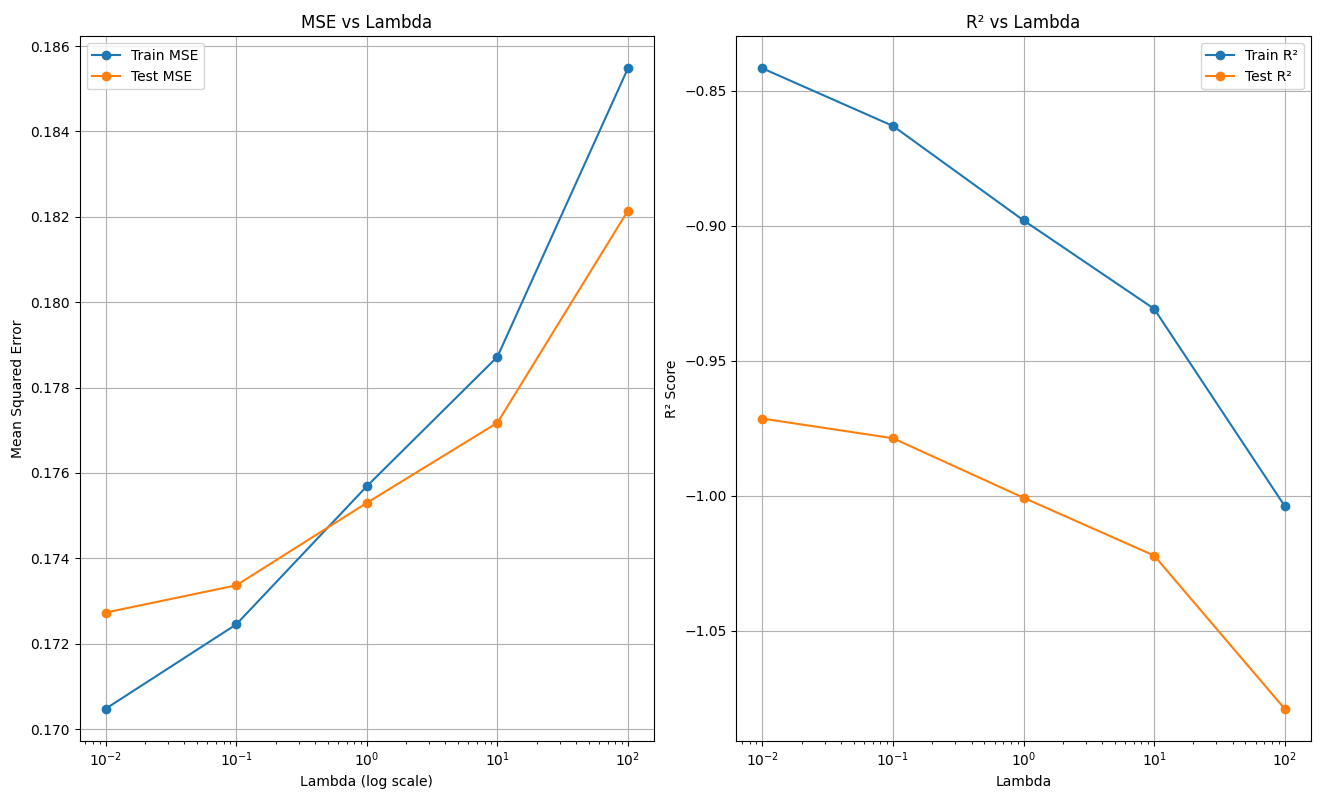
\includegraphics[width=1\textwidth]{Ridge_mse_r2.png}
    \newline
    \caption{Figure 8: MSE and R2 for training and test sets as a function of lambda}



\subsubsection{Mean Squared Error}

From Figure 8, we observe that the training MSE increases as \( \lambda \) increases. This is expected, as the increasing regularization term shrinks the magnitude of the regression coefficients, reducing the model's ability to fit the training data closely. For smaller values of \( \lambda \), the training error is low, indicating a good fit to the training data. However, as \( \lambda \) increases, the model becomes less flexible and underfits the data, leading to higher training errors. For testing data we observe a similar trend but with a lower rate of change.


\subsubsection{R2 Score}

Figure 8 shows the R2 score as a function of \( \lambda \). For the training data, the R2 score decreases monotonically with increasing \( \lambda \), consistent with the increase in training error. At small values of \( \lambda \), the model achieves a high R2 score on the training data, but this comes at the cost of overfitting, as seen by the lower R2 score on the test data.

For the test data, the R2 score shows a similar trend. The R2 score consistently decline, indicating that the model begins to underfit the test data due to excessive regularization.

\subsubsection{Optimal Value of \( \lambda \)}

The optimal regularization parameter \( \lambda \) was found to be the smallest \( \lambda \) in our interval. This supposes that we the range in which we tested \( \lambda \) values where to big. Too large \( \lambda \) values generalizes the model too much and negatively impacts both the training and testing MSE.


\subsection{Lasso regression}


To analyze the effectiveness of the Lasso regression method, it is important to observe how the Mean Squared Error (MSE) and \(R^2\) scores change across different values of lambda. \\

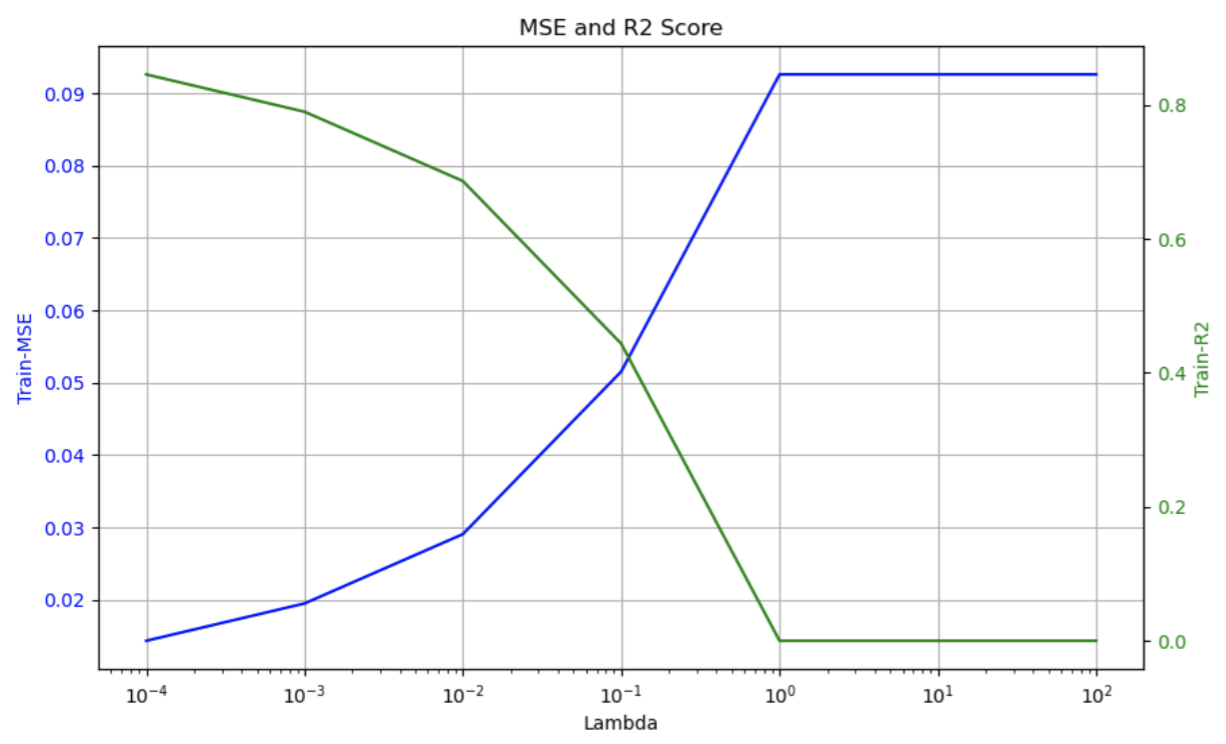
\includegraphics[width=1\linewidth]{imageLassoMSER2.png}
    \caption{Figure 9: Lasso Regression: MSE and R2 scores for different values of \(\lambda\)}
    \label{fig:enter-label}\\

Figure 9 illustrates the relationship between these metrics and lambda, where increasing lambda values lead to a rise in MSE and a decrease in \(R^2\). As lambda increases, Lasso penalizes larger coefficients more strongly, ultimately shrinking many of them toward zero, like seen in figure 11:\\

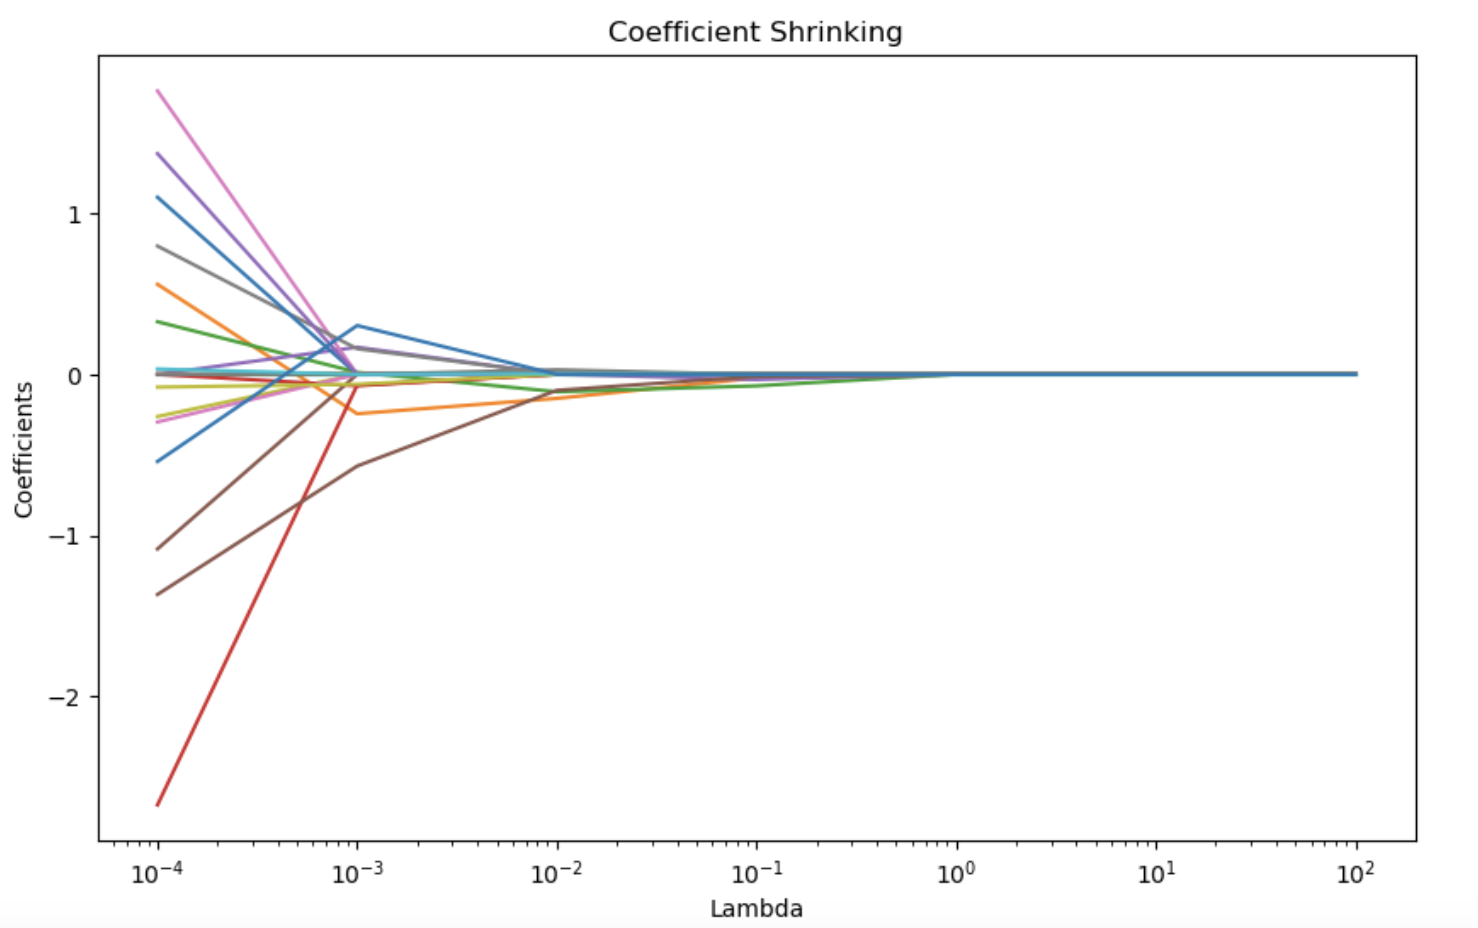
\includegraphics[width=1\linewidth]{imageLassoShrinkage.png}
    \caption{Figure 10: Coefficient shrinking for different values of lambda}
    \label{fig:enter-label}\\

The crossover point between the MSE and \(R^2\) curves highlights the impact of regularization strength on model performance. Identifying an optimal lambda is essential to balance underfitting and overfitting, which cannot be determined analytically but must be evaluated empirically, as shown in figure 10. Looking at it, one can see that an optimal lambda value would lie in the range of \((10^{-2}, 10^{-1})\), as it is in this range you get a model that is not overfitted, while still explaining the variance of the data. \\

\subsubsection{Comparing Lasso with Ridge and OLS Regression}

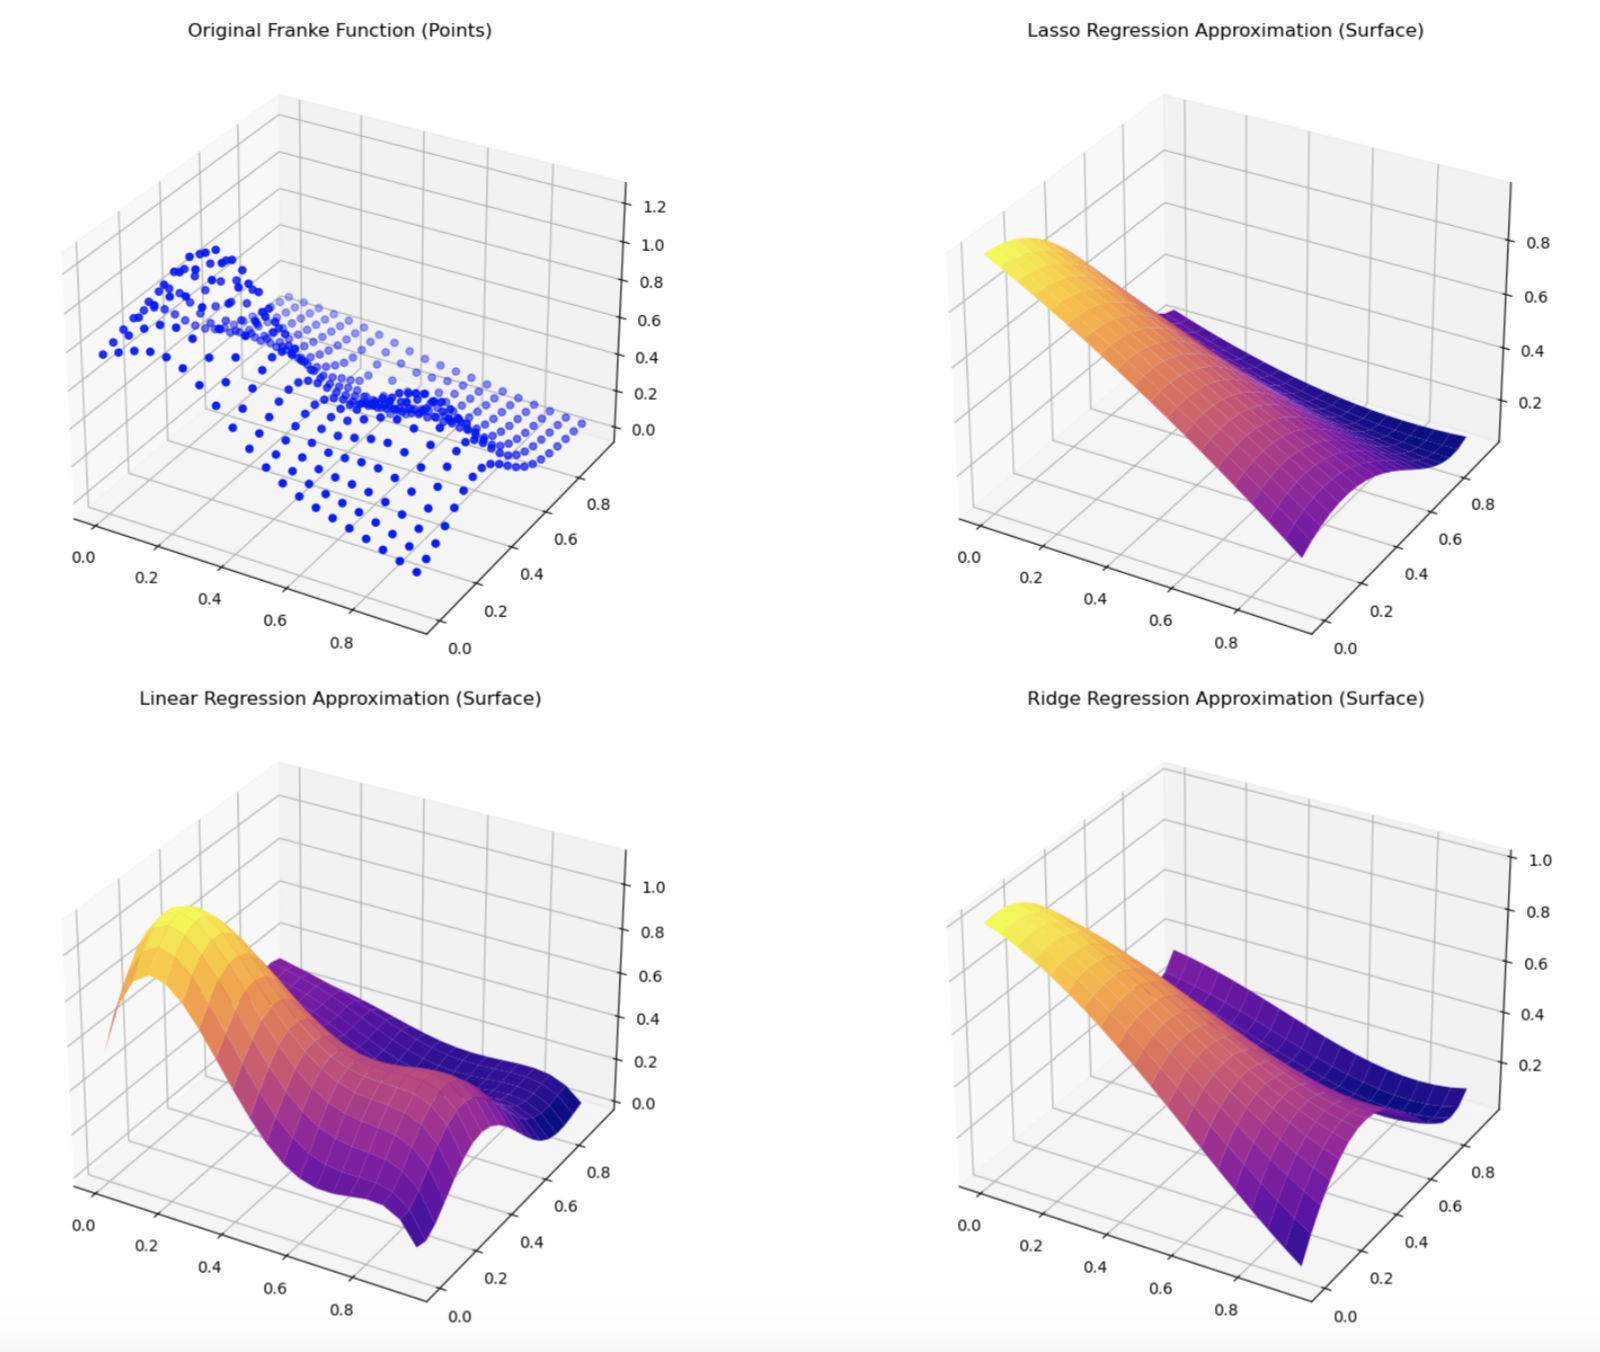
\includegraphics[width=1\linewidth]{imageRegComparison.png}
\caption{Figure 11: Visualization of the different prediction models as compared to the original franke function : tuned lasso}
\label{fig:enter-label}\\

Figure 11 visualizes how different prediction models approximate data generated by the Franke function. It is evident that the Lasso model struggles to capture the detailed features of the data, even when fine-tuned (
\(\lambda\)=0.01). Instead of capturing the nuanced variations, Lasso only grasps the broad strokes of variance in the z-values. This is likely a consequence of its L1 regularization, which, as discussed earlier, pushes some coefficients toward zero. In the context of topographical data analysis, where many features can be crucial, this level of simplification may lead to the loss of important characteristics, making Lasso less suitable for this type of analysis.\\

Ridge regression, on the other hand, performs slightly better by capturing some of the peaks and valleys of the Franke function. However, the model still produces a highly generalized surface, smoothing over many of the finer details and reducing the variance between extreme values. Like Lasso, Ridge also appears underfitted for this problem, lacking the necessary complexity to accurately predict the full range of z-values. This suggests that both Lasso and Ridge, while useful for avoiding overfitting, may not be well-suited for modeling real-world topographical data where capturing subtle features is important.\\

Ordinary Least Squares (OLS) regression appears to offer the best performance among the three models. As seen in figure 11, its surface follows the variations in the Franke function data more closely than either Lasso or Ridge. However, similar to the regularized models, OLS still fails to capture every fine detail of the original function. While it provides a better fit, OLS is not immune to the limitations of linear models, especially when approximating highly non-linear surfaces like the Franke function.

\subsection{Statistical interpretation of LR}
The primary focus was on deriving the expectation values and the variance for the estimated coefficient under Ordinary Least Squares (OLS) and the regression methods. 

\begin{enumerate}
    \item \textbf{Expectation of $y_i$:} It was shown that the expectation of $y_i$, given by $ y_i = X_i \beta + \epsilon_i $, is:
    \[
    E(y_i) = X_i \beta
    \]

This confirms that the expected value of each observation is determined by the linear model. 

    \item \textbf{Variance of $y_i$:} The variance of $y_i$ was derived as:
    \[
    \text{Var}(y_i) = \sigma^2
    \]

This implies that all observations have the same variance, corresponding to the noise in the model, which is $\sigma^2$.

    \item \textbf{Expectation of $\hat{\beta}$:} The OLS estimate $\hat{\beta}$ was shown to be an unbiased estimator:
    \[
    E(\hat{\beta}) = \beta
    \]

This means the OLS estimates are expected to be centered around the true parameter values. 
    \item \textbf{Variance of $\hat{\beta}$:} The variance of $\hat{\beta}$ was calculated as:
    \[
    \text{Var}(\hat{\beta}) = \sigma^2 (X^T X)^{-1}
    \]

This provides the dispersion of the estimated coefficients around the true values.  \end{enumerate}

\begin{enumerate}
    \item \textbf{Expectation of $\hat{\beta}_{\text{Ridge}}$:} The expectation of the Ridge regression estimator was derived as:
    \[
    E(\hat{\beta}_{\text{Ridge}}) = (X^T X + \lambda I)^{-1} X^T X \beta
    \]
    Unlike OLS, Ridge regression introduces bias into the estimates, as the expected value is not exactly $\beta$ for $\lambda > 0$.
    
    \item \textbf{Variance of $\hat{\beta}_{\text{Ridge}}$:} The variance of the Ridge regression coefficients was found to be:
    \[
    \text{Var}(\hat{\beta}_{\text{Ridge}}) = \sigma^2 (X^T X + \lambda I)^{-1} X^T X (X^T X + \lambda I)^{-1}
    \]

    The variance decreases as $\lambda$ increases, indicating that the estimates become more stable but at the cost of increased bias.
    
    \item \textbf{Effect of $\lambda$ on Variance:} As $\lambda \to \infty$, the variance of $\hat{\beta}_{\text{Ridge}}$ approaches zero:
    \[
    \text{Var}(\hat{\beta}_{\text{Ridge}}) \to 0 \quad \text{as} \quad \lambda \to \infty
    \]
    This demonstrates the bias-variance tradeoff inherent in Ridge regression, where larger regularization parameters stabilize the estimates but introduce more bias.
\end{enumerate}

The exercises highlighted the trade-offs between bias and variance in OLS and Ridge regression. While OLS provides unbiased estimates, Ridge regression reduces variance at the cost of introducing bias, demonstrating a fundamental aspect of regularization in statistical modeling.
\newpage
\subsection{Bias variance tradeoff using bootstrap}
We analyzed the Ordinary Least Squares (OLS) using \texttt{LinearRegression()}:

\subsubsection{Visualization and Analysis}

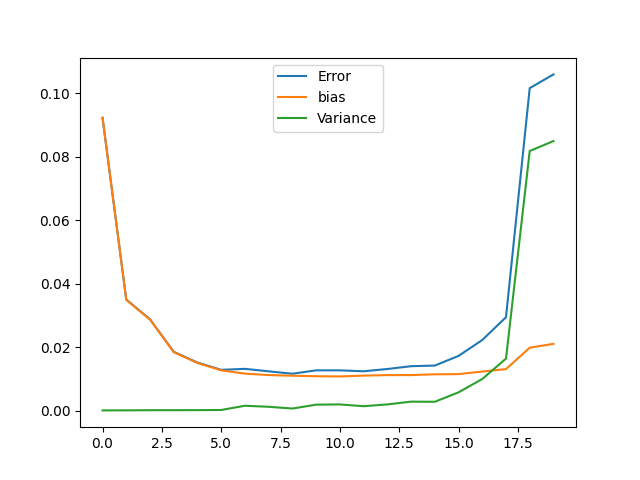
\includegraphics[width=1\linewidth]{bias_variance.png}
\caption{Figure 12: MSE, Bias and variance for different polynomial degrees }
\label{fig:enter-label}\\
    
After computing the bias, variance, and MSE for each polynomial degree, we plotted these quantities against the model complexity. This visualization helped us observe the tradeoff between bias and variance:

\begin{itemize} \item \textbf{Bias:} Generally decreases with increasing model complexity, as the model becomes more flexible and can better fit the true data. \item \textbf{Variance:} Generally increases with increasing model complexity, as the model becomes more sensitive to fluctuations in the training data. \item \textbf{MSE:} The sum of bias squared and variance, indicating the total expected prediction error. \end{itemize}

\subsubsection{Interpreting the Bias-Variance Tradeoff}

By analyzing the plots, we identified the polynomial degree at which the MSE is minimized, representing the optimal balance between bias and variance. This degree indicates the model complexity that achieves the best generalization performance on unseen data.
\newline\newline




\paragraph{Key Observations}

\begin{enumerate} 
\item \textbf{Low-Degree Polynomials:} High bias due to underfitting; the model is too simple to capture the underlying structure. 
\item \textbf{High-Degree Polynomials:} High variance due to overfitting; the model captures noise in the training data. 
\end{enumerate}


Through this bias-variance analysis, we systematically investigated how model complexity and regularization techniques affect the performance of regression models on the Franke Function. This methodology provides a framework for selecting models that achieve an optimal tradeoff, enhancing their predictive capabilities on new data.


\subsubsection{Impact of Number of Data Points}

The bias-variance tradeoff is not only influenced by model complexity but also by the amount of available data. As we increase the number of data points, the variance of the model tends to decrease, since the model becomes less sensitive to fluctuations in any single subset of the data. On the other hand, bias remains largely unaffected by the number of data points, as it is primarily dependent on the model's complexity.

\paragraph{Key Observations:}
\begin{enumerate}
    \item \textbf{More Data Points:} As the number of data points increases, the model tends to exhibit lower variance because it becomes more stable across different samples. This can mitigate the overfitting problem, especially in high-degree polynomial models.
    \item \textbf{Fewer Data Points:} With fewer data points, the model is more prone to variance, as it can overfit the limited data, especially when the model complexity is high.
    \item \textbf{Bias:} Increasing the number of data points does not significantly affect bias, as the bias is determined by how well the model structure captures the true underlying relationship, which is a function of the model complexity rather than the data size.
\end{enumerate}

Thus, increasing the data points typically helps to reduce the variance without impacting bias, resulting in improved generalization. This insight emphasizes the importance of having sufficient data when training complex models to control the variance while maintaining a low bias.

\subsection{k-fold cross validation}

The results of applying K-fold cross-validation to different regression models showed that increasing the number of folds did not significantly affect the MSE score. Validating the previous results and showing that the models are not overfitted. This implies that the models are generalized , explaining the absent variance in the resulting MSE scores. Figure 13 illustrates how little the MSE varies with different values of k:\\

\includegraphics[width=1\linewidth]{imageCrossValMSE.png}
\caption{Figure 113: Cross-validation: MSE for different values of k, Lasso : not tuned}
\label{fig:enter-label}\\

According to the results, Ordinary Least Squares (OLS) and Ridge regression models performed well on this dataset, while the Lasso regression exhibited poor performance. One potential reason for Lasso’s underperformance could be excessive penalization of important features, which reduces the accuracy of the model. Applying the principles learned in the lasso regression analysis, one can tune the \(\lambda\) parameter to better the model. Setting the \(\lambda\) value to 0.01, instead of the default 0.1, you get:\\

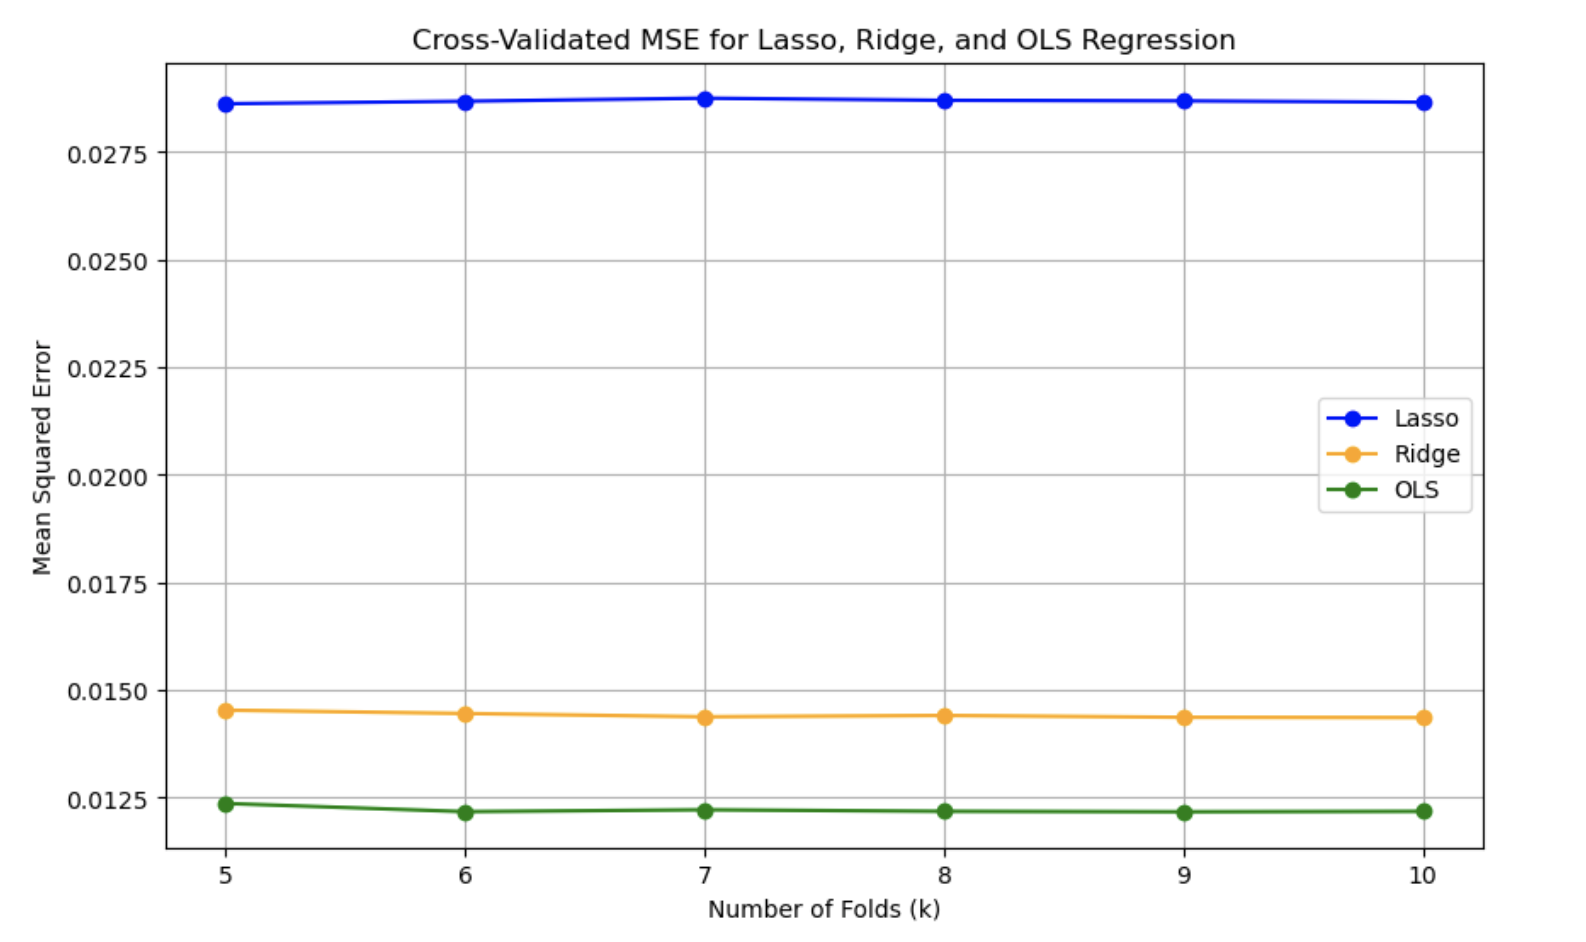
\includegraphics[width=1\linewidth]{imageLassoK-fold2.png}
\caption{Figure 14: Cross-validation: MSE for different values of k, Lasso : tuned}
\label{fig:enter-label}\\

While tuning the \(\lambda\) parameter improved Lasso’s performance, both OLS and Ridge regression still outperformed the Lasso model. This suggests that for this particular dataset, Lasso’s strength in feature selection may not be as beneficial, and the regularization it imposes might be too restrictive, even after tuning. Further tuning or adjusting the data preprocessing steps (e.g., scaling or feature transformation) could potentially enhance Lasso’s performance, though Ridge and OLS appear to be better suited to this dataset overall, as they are shown to not be over fitted.

\subsubsection{Comparing Bootstrap and k-fold Cross-validation}

\paragraph{Bootstrap}
Bootstrap resampling provides a direct estimate of model variance by generating multiple training sets from the original sample, making it effective for small datasets or when a single train-test split may not be representative. It captures model variability well but can over-represent certain data points due to sampling with replacement, potentially inflating variance estimates.

\paragraph{K-fold cross validation}
splits the dataset into k subsets, ensuring each data point serves as a test set once. It is more computationally efficient than bootstrap, particularly for larger datasets, and avoids the redundancy of resampling. Our analysis showed that increasing the number of folds had little effect on MSE, confirming the generalization and robustness of OLS and Ridge models.
\newline\newline

Overall, K-fold produced more stable and slightly lower MSEs than bootstrap. Both methods affirmed that OLS and Ridge outperformed Lasso, with Lasso showing higher variance and sensitivity to regularization tuning.

\section{Discussion}

In this study, polynomial regression models (OLS, Ridge, and Lasso) were applied to predict terrain data from Norway. While the methods captured broad trends in the data, there were notable limitations and areas where the models underperformed. This section critically assesses the strengths and weaknesses of the approach, placing the results in the context of machine learning methods for regression, and offers insights for future improvements.

\subsection{Model Performance and Analysis}

The primary evaluation metric used to assess model performance was the Mean Squared Error (MSE). The results for OLS, Ridge, and Lasso were relatively consistent, with OLS and Ridge showing near-identical MSE values (~29,444), while Lasso exhibited a significantly higher MSE (~31,734). These values suggest several key points about the models' ability to capture the underlying terrain data:\\

OLS and Ridge Regularization: The minimal difference in MSE between OLS and Ridge indicates that Ridge's regularization had little to no effect in this specific context. Regularization is generally applied to prevent overfitting, but in this case, the data and design matrix did not introduce enough variance or noise for regularization to significantly improve the performance. This suggests that OLS was already well-suited to the problem at hand, and the data was not overfitted, meaning that the addition of a penalty term for Ridge was not necessary.\\
    
Lasso's Poor Performance: Lasso, on the other hand, underperformed with a higher MSE value, despite its ability to shrink coefficients. This was likely due to Lasso's over-regularization, which caused it to zero out coefficients that may have been important in capturing the finer details of the terrain. The sparse nature of Lasso regression makes it well-suited for datasets with many irrelevant features, but for this dataset where the features are generated from a polynomial design matrix Lasso's simplification caused the model to lose valuable information about the terrain's complexity.\\


These results align with the literature on the limitations of Lasso in highly structured datasets, such as those produced by polynomial features. Ridge, which retains all coefficients but penalizes large values, performs better in such contexts, although in this case, the gains were marginal due to the relatively low complexity of the dataset.

\subsection{Visual Results and Interpretation}

The visualizations of the terrain predictions provided additional insights into how well the models captured the underlying patterns in the data. While the OLS and Ridge models were able to approximate the general shape of the terrain, both models produced overly smooth surfaces that lacked the sharp peaks and valleys characteristic of the real-world terrain data. The OLS-predicted surface, for example, smoothed out finer details, indicating that the polynomial degree of 5 might not have been sufficient to capture the high-frequency variations present in the data.


\includegraphics[width=1\linewidth]{10.png}
\caption{Figure 15: OLS Prediction (Degree 5)}
\label{fig:enter-label}\\


The lack of fine details in the OLS and Ridge predictions highlights a key limitation of using low-degree polynomial regression. Although the MSE values indicated decent performance, the models failed to represent the detailed variations in the terrain. This underfitting problem could potentially be addressed by increasing the polynomial degree, but doing so comes with the risk of overfitting, especially if the model becomes too complex relative to the size of the training data.

\includegraphics[width=1\linewidth]{9.png}
\caption{Figure 16: Original Terrain}
\label{fig:enter-label}\\


The visual comparison between the original terrain and the OLS-predicted terrain clearly shows that the predicted surface is much smoother and misses the detailed peaks and valleys observed in the original data. \cite{bishop2006pattern}



\subsection{Effectiveness of Cross-Validation}

The use of 5-Fold Cross-Validation confirmed that the OLS and Ridge models generalized well across different data splits, with consistent MSE values across the folds. The slight difference between the cross-validated MSE values for OLS and Ridge (29473 vs 29474) reinforces the earlier conclusion that Ridge's regularization provided minimal benefits. This suggests that the variance in the data was low enough that OLS was able to generalize effectively without requiring any regularization.\\

On the other hand, Lasso’s cross-validated MSE (~31,760) was considerably higher than OLS and Ridge, further validating its tendency to oversimplify the model by eliminating too many coefficients. This behavior of Lasso aligns with known issues in terrain modeling and other datasets where many features are relevant and removing them leads to underfitting.

\subsection{Limitations and Future Directions}

Several limitations became apparent during this study, providing avenues for future improvements:

\begin{itemize}
    \item \textbf{Polynomial Degree}: The polynomial degree chosen (5) may have been too low to capture the intricacies of the terrain. A higher polynomial degree could better model the sharp variations in the data, though it risks overfitting. Future work could explore cross-validation or information criteria (e.g., AIC, BIC) to select the optimal polynomial degree, balancing bias and variance.
    
    \item \textbf{Model Selection}: While this study was limited to OLS, Ridge, and Lasso, more advanced models such as decision trees, random forests, or neural networks may provide superior performance in terrain modeling tasks. These models are better suited for capturing complex, nonlinear relationships and do not require feature engineering via polynomial expansions. Neural networks, for example, could potentially learn intricate patterns from the terrain data without relying on predefined polynomial terms.
    
    \item \textbf{Feature Scaling and Tuning}: Although the data was standardized for Ridge and Lasso, more careful tuning of the regularization parameters (e.g., alpha) could lead to better results. A comprehensive grid search or random search over hyperparameters could further improve Ridge and Lasso's performance, especially if the terrain data presents subtle nonlinear relationships.
    
    \item \textbf{Data Resolution}: The resolution of the terrain data itself could influence model performance. Finer resolution data could lead to better predictions but would also require more complex models capable of handling such data. In this study, the polynomial degree may not have been sufficient to fully exploit the available data's resolution.
\end{itemize}

\subsection{Context and Relevance of the Work}

This work fits into the broader context of regression analysis applied to geographical and terrain data. Polynomial regression is a common approach for fitting surface data due to its simplicity and interpretability. However, the findings of this study highlight the limitations of classical regression methods in modeling complex, real-world terrain data. Specifically, terrain data often contain high-frequency variations that are difficult to capture with low-degree polynomials or simple regularized linear models.\\

In practical applications, more sophisticated machine learning algorithms such as neural networks or ensemble methods might be more appropriate for high-resolution terrain data. These models can automatically capture complex nonlinearities without requiring explicit polynomial feature engineering. Nonetheless, this study demonstrates the value of regression models as a baseline approach, providing insights into how regularization affects performance in the context of smooth surfaces like terrain.\\

In conclusion, the analysis showed that while OLS and Ridge regression provided reasonable approximations of the terrain, both models were limited in capturing finer details. Lasso, due to its aggressive regularization, underperformed, indicating that terrain modeling requires preserving coefficients that contribute to the complexity of the surface. The visualizations underscored the need for higher-order polynomials or more advanced models to capture the full range of variations present in the terrain. Cross-validation further validated the robustness of OLS and Ridge, but more sophisticated models may be required to fully capture the terrain’s complexity.

\section{Conclusion}

The objective of this study was to analyze and compare the performance of three regression methods—Ordinary Least Squares (OLS), Ridge, and Lasso—on both synthetic data generated by the Franke Function and real-world terrain data. Using metrics such as Mean Squared Error (MSE) and \( R^2 \) scores, along with resampling techniques like Bootstrap and K-fold cross-validation, we evaluated each model's ability to generalize and capture underlying patterns in the data.\\

Our main findings indicate that OLS and Ridge regression effectively modeled datasets of moderate complexity. OLS served as a solid baseline, providing good fits to the data but showing susceptibility to overfitting, especially with higher-degree polynomials and noisy data. Ridge regression, with its \( L2 \) regularization, mitigated overfitting by shrinking coefficient magnitudes, resulting in better generalization on both synthetic and real-world datasets. Conversely, Lasso regression underperformed due to its aggressive \( L1 \) regularization, which excessively penalized important features and led to underfitting—particularly evident in the complex terrain data where it failed to capture crucial details.\\

Interpreting these results, we observe that while regularization is essential for controlling overfitting, the choice between \( L1 \) and \( L2 \) penalties significantly impacts model performance. Ridge's ability to retain all features while reducing their impact proved advantageous for datasets where every feature contributes meaningfully. Lasso's feature selection capabilities are beneficial in high-dimensional spaces with many irrelevant features but can be detrimental when important features are penalized too harshly.\\

Looking ahead, several avenues for future work present themselves. One potential improvement is to explore higher-degree polynomial models or interaction terms to better capture the nonlinearities inherent in complex datasets like terrain data. 

Discussing the pros and cons of the methods, OLS is straightforward and interpretable but prone to overfitting complex data. Ridge regression offers a balance by reducing overfitting without eliminating features, making it suitable for datasets with multicollinearity. Lasso regression excels in feature selection but may underfit when all features are relevant, as seen in our terrain analysis. \\

In conclusion, selecting a regression method that aligns with the complexity and characteristics of the data is crucial. While OLS and Ridge showed competence in handling moderate complexities, their limitations—especially in capturing the finer details of real-world terrain—highlight the need for more sophisticated models. Future work should focus on integrating more flexible, non-linear methods and performing thorough hyperparameter tuning to enhance model performance in complex, real-world applications.
 

\bibliographystyle{plain}
\bibliography{bib}


\end{document}
